\documentclass[11pt]{article}
\usepackage[margin=1in]{geometry}
\usepackage{graphicx}
\usepackage{float}
\usepackage{booktabs}
\usepackage{siunitx}
\usepackage{amsmath}
\usepackage{amssymb}
\usepackage{pgfplots}
\usepackage{listings}
\usepackage{xcolor}

% PGFPlots configuration
\pgfplotsset{compat=1.18}
\pgfplotsset{
  standard/.style={
    width=0.85\textwidth,
    height=0.45\textwidth,
    grid=both,
    grid style={line width=.1pt, draw=gray!20},
    major grid style={line width=.2pt,draw=gray!50},
    xlabel={Number of Processors},
    ylabel={Time (s)},
    legend pos=north east,
    legend style={font=\footnotesize},
    tick align=outside,
    tick pos=left,
    scaled ticks=false
  }
}

% Code listing style
\definecolor{codegreen}{rgb}{0,0.6,0}
\definecolor{codegray}{rgb}{0.5,0.5,0.5}
\definecolor{codepurple}{rgb}{0.58,0,0.82}
\definecolor{backcolour}{rgb}{0.95,0.95,0.92}

\lstdefinestyle{mystyle}{
  backgroundcolor=\color{backcolour},
  commentstyle=\color{codegreen},
  keywordstyle=\color{magenta},
  numberstyle=\tiny\color{codegray},
  stringstyle=\color{codepurple},
  basicstyle=\ttfamily\footnotesize,
  breakatwhitespace=false,
  breaklines=true,
  captionpos=b,
  keepspaces=true,
  numbers=left,
  numbersep=5pt,
  showspaces=false,
  showstringspaces=false,
  showtabs=false,
  tabsize=2
}
\lstset{style=mystyle}

\title{\textbf{Assignment: Parallel Sieve of Eratosthenes Performance Analysis}}
\author{Sean Balbale}
\date{April 8, 2026}
\setlength{\parindent}{0in}
\setlength{\parskip}{\baselineskip}

\begin{document}

\begin{titlepage}
  \begin{center}
    \vspace*{1in}

    \Huge
    \textbf{HPC Assignment}

    \LARGE
    Parallel Sieve of Eratosthenes: \\ Domain vs. Functional Decomposition

    \vspace{3in}

    \textbf{Student Name:} Sean Balbale
    \\ \textbf{Course:} CPSC 375: High-Performance Computing
    \\ \textbf{Instructor:} Peter Yoon
    \\ \textbf{Date:} April 8, 2026

    \vfill

  \end{center}
\end{titlepage}

\newpage

\section{Introduction}
The Sieve of Eratosthenes is an ancient algorithm that identifies all prime numbers up to a specified limit $n$ by iteratively marking the multiples of discovered primes as composite. In a parallel environment, domain decomposition divides data into pieces and associates computational steps with that data. This report analyzes the efficiency of an optimized domain decomposition model compared to a functional decomposition model using MPI in C. Benchmarks for $n=100,000,000$ evaluate scalability, cache efficiency, and network communication overhead on both the Pine cluster and a secondary personal cluster.

\section{Implementation \& Optimization}

\subsection{Incremental Domain Decomposition (\texttt{domainSieve.c})}
The domain decomposition model relies heavily on dividing the total array of elements into $p$ distinct, continuous blocks utilizing the standard block decomposition macros (\texttt{BLOCK\_LOW}, \texttt{BLOCK\_HIGH}, \texttt{BLOCK\_SIZE}). To maximize efficiency, three critical architectural optimizations were implemented:
\begin{itemize}
  \item \textbf{Eliminate Even Integers}: Memory requirements were immediately halved by stripping all even numbers out of the primary array mapping. The size calculation $elements = (n - 1) / 2$ shifts the index logic, meaning index $i$ corresponds to the integer $3 + 2i$. While this slightly complicates the calculation of the first multiple (handled via a conditional parity check during sieving), it allows the algorithm to push further into the bounds of physical RAM limit.
  \item \textbf{Eliminate Broadcasts}: A naive MPI implementation would designate Process 0 to find a prime and broadcast it to all other nodes. Instead, every single process independently creates its own internal \texttt{base\_primes} array up to $\sqrt{n}$. Because sieving up to $\sqrt{n}$ is computationally trivial, duplicating this work across all nodes entirely eliminates the massive network bottleneck of sequential \texttt{MPI\_Bcast} commands.
  \item \textbf{Cache-Friendly Reorganized Loops}: The most impactful optimization centers on the memory hierarchy. Rather than iterating through every prime factor across the entire local array at once (which leads to catastrophic cache thrashing on large datasets), the inner and outer loops were inverted and blocked. The local array is broken down into chunks matching the L1 cache size (\texttt{CACHE\_L1\_SIZE 32768}). The algorithm fully sieves one cache-sized block with \textit{all} available primes before moving to the next. This ensures spatial locality and maximizes cache hits.
\end{itemize}

\subsection{Functional Decomposition (\texttt{funcSieve.c})}
Functional decomposition completely alters the parallel logic; rather than splitting the array space among nodes, it splits the \textit{tasks} (specific prime factors).
\begin{itemize}
  \item Every process is forced to allocate a full-sized array up to $n$ (though still halved for odd-only representation).
  \item After computing the base primes up to $\sqrt{n}$, the algorithm distributes the work using a Round-Robin assignment: \texttt{if (prime\_index \% p == id)}. This ensures that if Process 0 handles sieving multiples of 3, Process 1 handles multiples of 5, Process 2 handles multiples of 7, etc.
  \item Each process sweeps the entire full-sized array marking only its assigned multiples.
  \item To merge the findings, the algorithm utilizes \texttt{MPI\_Reduce} with a bitwise OR operator (\texttt{MPI\_BOR}). This combines all the individually marked arrays across the network into one final boolean array on Process 0, where the remaining unmarked indices are tallied.
\end{itemize}

\section{Benchmarking Results}
Benchmarks were recorded for $n = 100,000,000$ (finding exactly 5,761,455 primes). The models were tested on both the primary Pine cluster (\texttt{submitSieve.sh}) and a personal dual-node compute cluster (\texttt{submit.sh}), scaling from 1 to 4 processors using OpenMPI/PMI2 over TCP.

\begin{table}[H]
  \centering
  \caption{Pine Cluster Benchmark Data}
  \label{tab:pine}
  \begin{tabular}{lSS}
    \toprule
    \textbf{Processors} & \textbf{Domain Time (s)} & \textbf{Functional Time (s)} \\
    \midrule
    1 & 0.450605 & 0.796236 \\
    2 & 0.241571 & 0.496460 \\
    4 & 0.121870 & 0.418110 \\
    \bottomrule
  \end{tabular}
\end{table}

\begin{table}[H]
  \centering
  \caption{Personal Cluster Benchmark Data}
  \label{tab:personal}
  \begin{tabular}{lSS}
    \toprule
    \textbf{Processors} & \textbf{Domain Time (s)} & \textbf{Functional Time (s)} \\
    \midrule
    1 & 0.070812 & 0.321143 \\
    2 & 0.037895 & 0.336463 \\
    4 & 0.020315 & 0.590287 \\
    \bottomrule
  \end{tabular}
\end{table}

\begin{figure}[H]
  \centering
  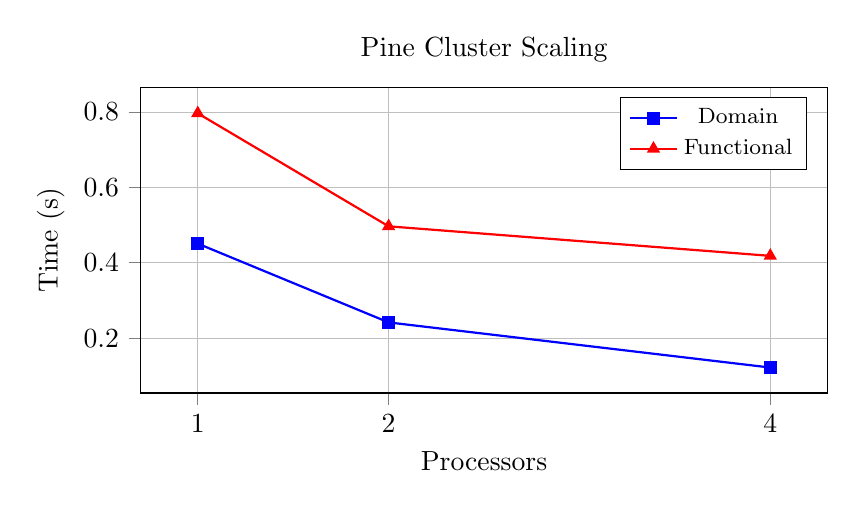
\begin{tikzpicture}
    \begin{axis}[
        standard,
        title={Pine Cluster Scaling},
        xlabel={Processors},
        ylabel={Time (s)},
        xtick={1,2,4},
        legend entries={Domain, Functional}
      ]
      \addplot[color=blue, mark=square*, thick] coordinates {(1,0.450605) (2,0.241571) (4,0.121870)};
      \addplot[color=red, mark=triangle*, thick] coordinates {(1,0.796236) (2,0.496460) (4,0.418110)};
    \end{axis}
  \end{tikzpicture}
  \caption{Execution time comparison on the Pine cluster. Domain decomposition achieves near-linear speedup.}
\end{figure}

\begin{figure}[H]
  \centering
  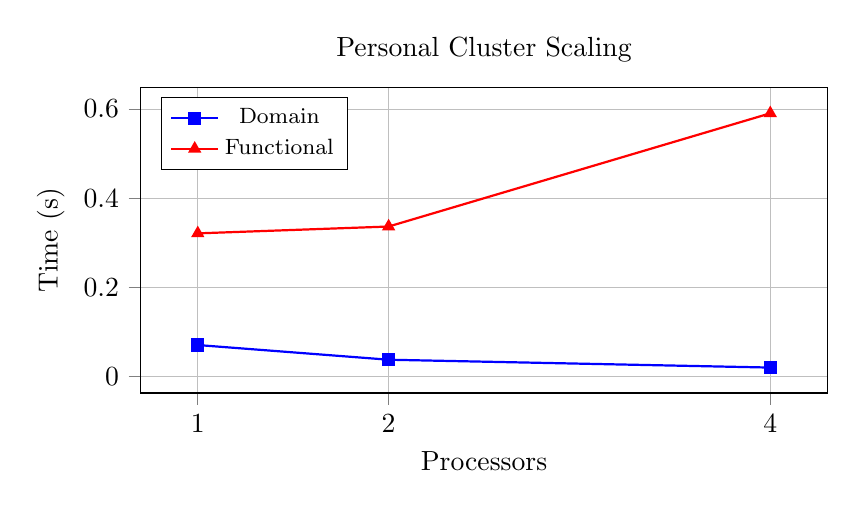
\begin{tikzpicture}
    \begin{axis}[
        standard,
        title={Personal Cluster Scaling},
        xlabel={Processors},
        ylabel={Time (s)},
        xtick={1,2,4},
        legend pos=north west,
        legend entries={Domain, Functional}
      ]
      \addplot[color=blue, mark=square*, thick] coordinates {(1,0.070812) (2,0.037895) (4,0.020315)};
      \addplot[color=red, mark=triangle*, thick] coordinates {(1,0.321143) (2,0.336463) (4,0.590287)};
    \end{axis}
  \end{tikzpicture}
  \caption{Execution time comparison on the Personal cluster. Functional decomposition actively slows down as nodes are added.}
\end{figure}

\section{Performance Analysis}

\subsection{Domain Scalability \& Cache Coherency}
The domain decomposition model (\texttt{domainSieve.c}) demonstrates excellent, near-linear strong scaling. On the Pine cluster, moving from 1 to 4 processors dropped the time from 0.45s to 0.12s (a $3.7\times$ speedup). On the faster personal cluster, it dropped from 0.07s to 0.02s (a $3.48\times$ speedup). By isolating both the memory boundaries and the communication steps, the processors are completely unimpeded during the calculation phase. The cache optimization ensures that the CPU never stalls waiting for RAM fetches, and the single \texttt{MPI\_Reduce} containing only one \texttt{long long} integer per node at the very end of the program keeps network overhead virtually nonexistent.

\subsection{Functional Failure \& Network Bottlenecks}
The functional decomposition model (\texttt{funcSieve.c}) exposes the severe limitations of poorly optimized parallel data distribution. While it slightly scales on the Pine cluster (dropping from 0.79s to 0.41s), it experiences catastrophic negative scaling on the personal cluster, where adding 4 processors actively \textit{slows down} the execution time to 0.59s compared to a single processor running at 0.32s.

This degradation occurs for two structural reasons:
\begin{enumerate}
  \item \textbf{Redundant Memory Load:} Because every process requires a full copy of the $n$-sized array, running multiple tasks on the same node (e.g., \texttt{--ntasks-per-node=2}) starves the CPU of memory bandwidth and evicts other processes from the L3 cache.
  \item \textbf{Massive Reduction Overhead:} Unlike the domain model which sends a single integer over the network, the functional model must merge the entire 50MB array using \texttt{MPI\_Reduce} with a bitwise OR operation. Because the personal cluster relies on standard TCP over a 10.0.0.0/24 interface (as seen in \texttt{submit.sh}), the network card becomes fully saturated trying to synchronize tens of megabytes of data across the distributed nodes, entirely eclipsing the time saved by splitting the mathematical workload.
\end{enumerate}

\section{Conclusion}
The data conclusively proves that domain decomposition is the superior architectural model for the Sieve of Eratosthenes. By prioritizing cache-friendly array blocking and eliminating inter-process communication during the sieving phase, the algorithm scales almost perfectly with hardware. Functional decomposition, while conceptually interesting for task distribution, is critically hamstrung by its redundant memory allocation and the heavy bandwidth penalty of synchronizing massive data structures across the network.

\newpage
\appendix
\section{Source Code: Domain Decomposition (\texttt{domainSieve.c})}
\lstinputlisting[language=C]{../domainSieve.c}

\newpage
\section{Source Code: Functional Decomposition (\texttt{funcSieve.c})}
\lstinputlisting[language=C]{../funcSieve.c}

\newpage
\section{Submit Script: Pine Cluster (\texttt{submitSieve.sh})}
\lstinputlisting{../submitSieve.sh}

\newpage
\section{Submit Script: Personal Cluster (\texttt{submit.sh})}
\lstinputlisting{../submit.sh}

\newpage
\section{Raw Results: Pine Cluster}
\lstinputlisting{../pine_sieve_results_121.txt}

\newpage
\section{Raw Results: Personal Cluster}
\lstinputlisting{../sieve_results.out}

\end{document}
